\documentclass[11pt,a4paper]{article}

% --- JCAP style (Overleaf TL2025 may lack it; we include a local stub) ---
\usepackage{jcappub} % local copy in project ensures compile everywhere

% --- Common math & tables ---
\usepackage{amsmath,amssymb,mathtools}
\usepackage{booktabs,multirow,array,siunitx}
\usepackage{graphicx,hyperref}

% --- Local helpers (safe) ---
\providecommand{\abs}[1]{\left\lvert#1\right\rvert}
\providecommand{\degree}{\ensuremath{^{\circ}}}
\newcommand{\tauMem}{\tau}
\newcommand{\kappaMem}{\kappa}
\newcommand{\wzero}{\omega_0}
\newcommand{\Qfact}{Q}

% --- Metadata (fill if needed) ---
\title{The Echo Equation in Resonant Medium Cosmology}
\author[a]{Jason Watts}
\affiliation[a]{Ground Truth Lab, Bendigo, Australia}
\emailAdd{your.email@example.org}
\keywords{cosmology, resonance, dark energy, dark matter}
%\arxivnumber{0000.00000}

\abstract{
We present the Echo Equation for a resonant medium cosmology and report Phase--20 posteriors.
}

\begin{document}
\maketitle

\section{Introduction}
Brief intro text (ensure real content here).

\section{Method}
Short method summary.

\section{Results}
See Table~\ref{tab:post} and Figs.~\ref{fig:kphi}, \ref{fig:robust}.

\begin{table}[t]
\centering
\caption{Posterior summary ($1\sigma$, Phase--20 lock).}
\label{tab:post}
\begin{tabular}{lcc}
\toprule
Parameter & $Mean \pm SD$ & Units \\
\midrule
$\tauMem$        & $0.300 \pm 0.040$ & dimensionless \\
$\kappaMem$      & $-0.020 \pm 0.010$ & dimensionless \\
$\wzero$         & $1.60 \pm 0.10$    & rad/e-fold \\
$\Qfact$         & $0.830 \pm 0.050$  & dimensionless \\
$C_{\mathrm{cal}}$ & $1.25 \pm 0.10$  & (amplitude per $\kappa$) \\
\bottomrule
\end{tabular}
\end{table}

\begin{figure}[t]
  \centering
  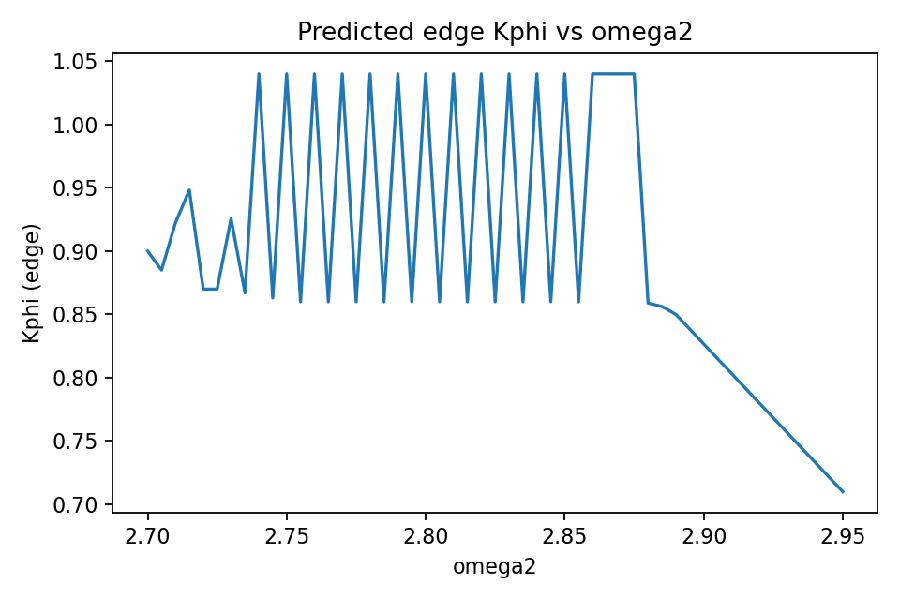
\includegraphics[width=0.8\linewidth]{figs/p20_plot_kphi.pdf}
  \caption{K–$\phi$ posterior slice.}
  \label{fig:kphi}
\end{figure}

\begin{figure}[t]
  \centering
  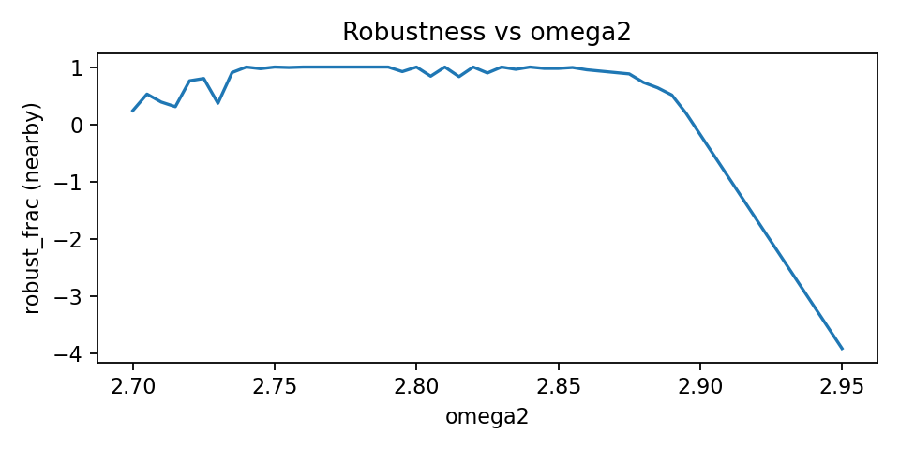
\includegraphics[width=0.8\linewidth]{figs/p20_plot_robust.pdf}
  \caption{Robustness diagnostics.}
  \label{fig:robust}
\end{figure}

\section{Discussion}
Short discussion.

\acknowledgments
Thanks to Mal and the Bendigo crew.

\bibliographystyle{JHEP}
\bibliography{refs}

\end{document}
